% !TeX root = ../../Skript.tex
\cohead{\Large\textbf{Nullstellen - näherungsweise}}
\fakesubsection{Nullstellen - näherungsweise}
Wir haben die Behauptung aufgestellt, dass sich Gleichungen vom Typ \(ae^{kx}+mx+b=0\) im Allgemeinen nicht exakt lösen lassen. Im Allgemeinen bedeutet, dass es durchaus Gleichungen dieses Typs gibt, die man exakt lösen kann, aber nicht jede Gleichung ist exakt lösbar. Als Beispiel betrachten wir \(f(x)=e^x+x-3\). Aus dem Schaubild lässt sich entnehmen, dass die Funktion eine Nullstelle im positiven Bereich haben muss. Zeichnet man das Schaubild mit dem Computer, so kann man sogar sagen, dass die Nullstellen zwischen \(x=0\) und \(x=1\) liegen muss. Dies könnte man auch mit dem Taschenrechner und einer Wertetabelle zeigen. Da \(f(0)=-2\) und \(f(1)\approx 0,72\) gilt, muss mindestens eine Nullstelle in diesem Bereich liegen.

\medskip

\begin{minipage}{\textwidth}
    \adjustbox{valign=t}{\begin{minipage}{0.5\textwidth}
            ACHTUNG: Wechseln die Funktionswerte einer Funktion ihr Vorzeichen, so kann man ohne weitere Überlegungen nur sagen, dass mindestens eine Nullstelle im fraglichen Bereich liegen muss, es könnten aber auch mehr Nullstellen sein. Findet kein Vorzeichenwechsel der Funktionswerte statt, kann man keine Aussage treffen. So hat \(x^2\) keinen Vorzeichenwechsel in den Funktionswerten, aber dennoch eine Nullstelle bei \(x=0\).
    \end{minipage}}%
    \adjustbox{valign=t, padding=2ex 0ex 0ex 0ex}{\begin{minipage}{0.5\textwidth-2ex}
        \centering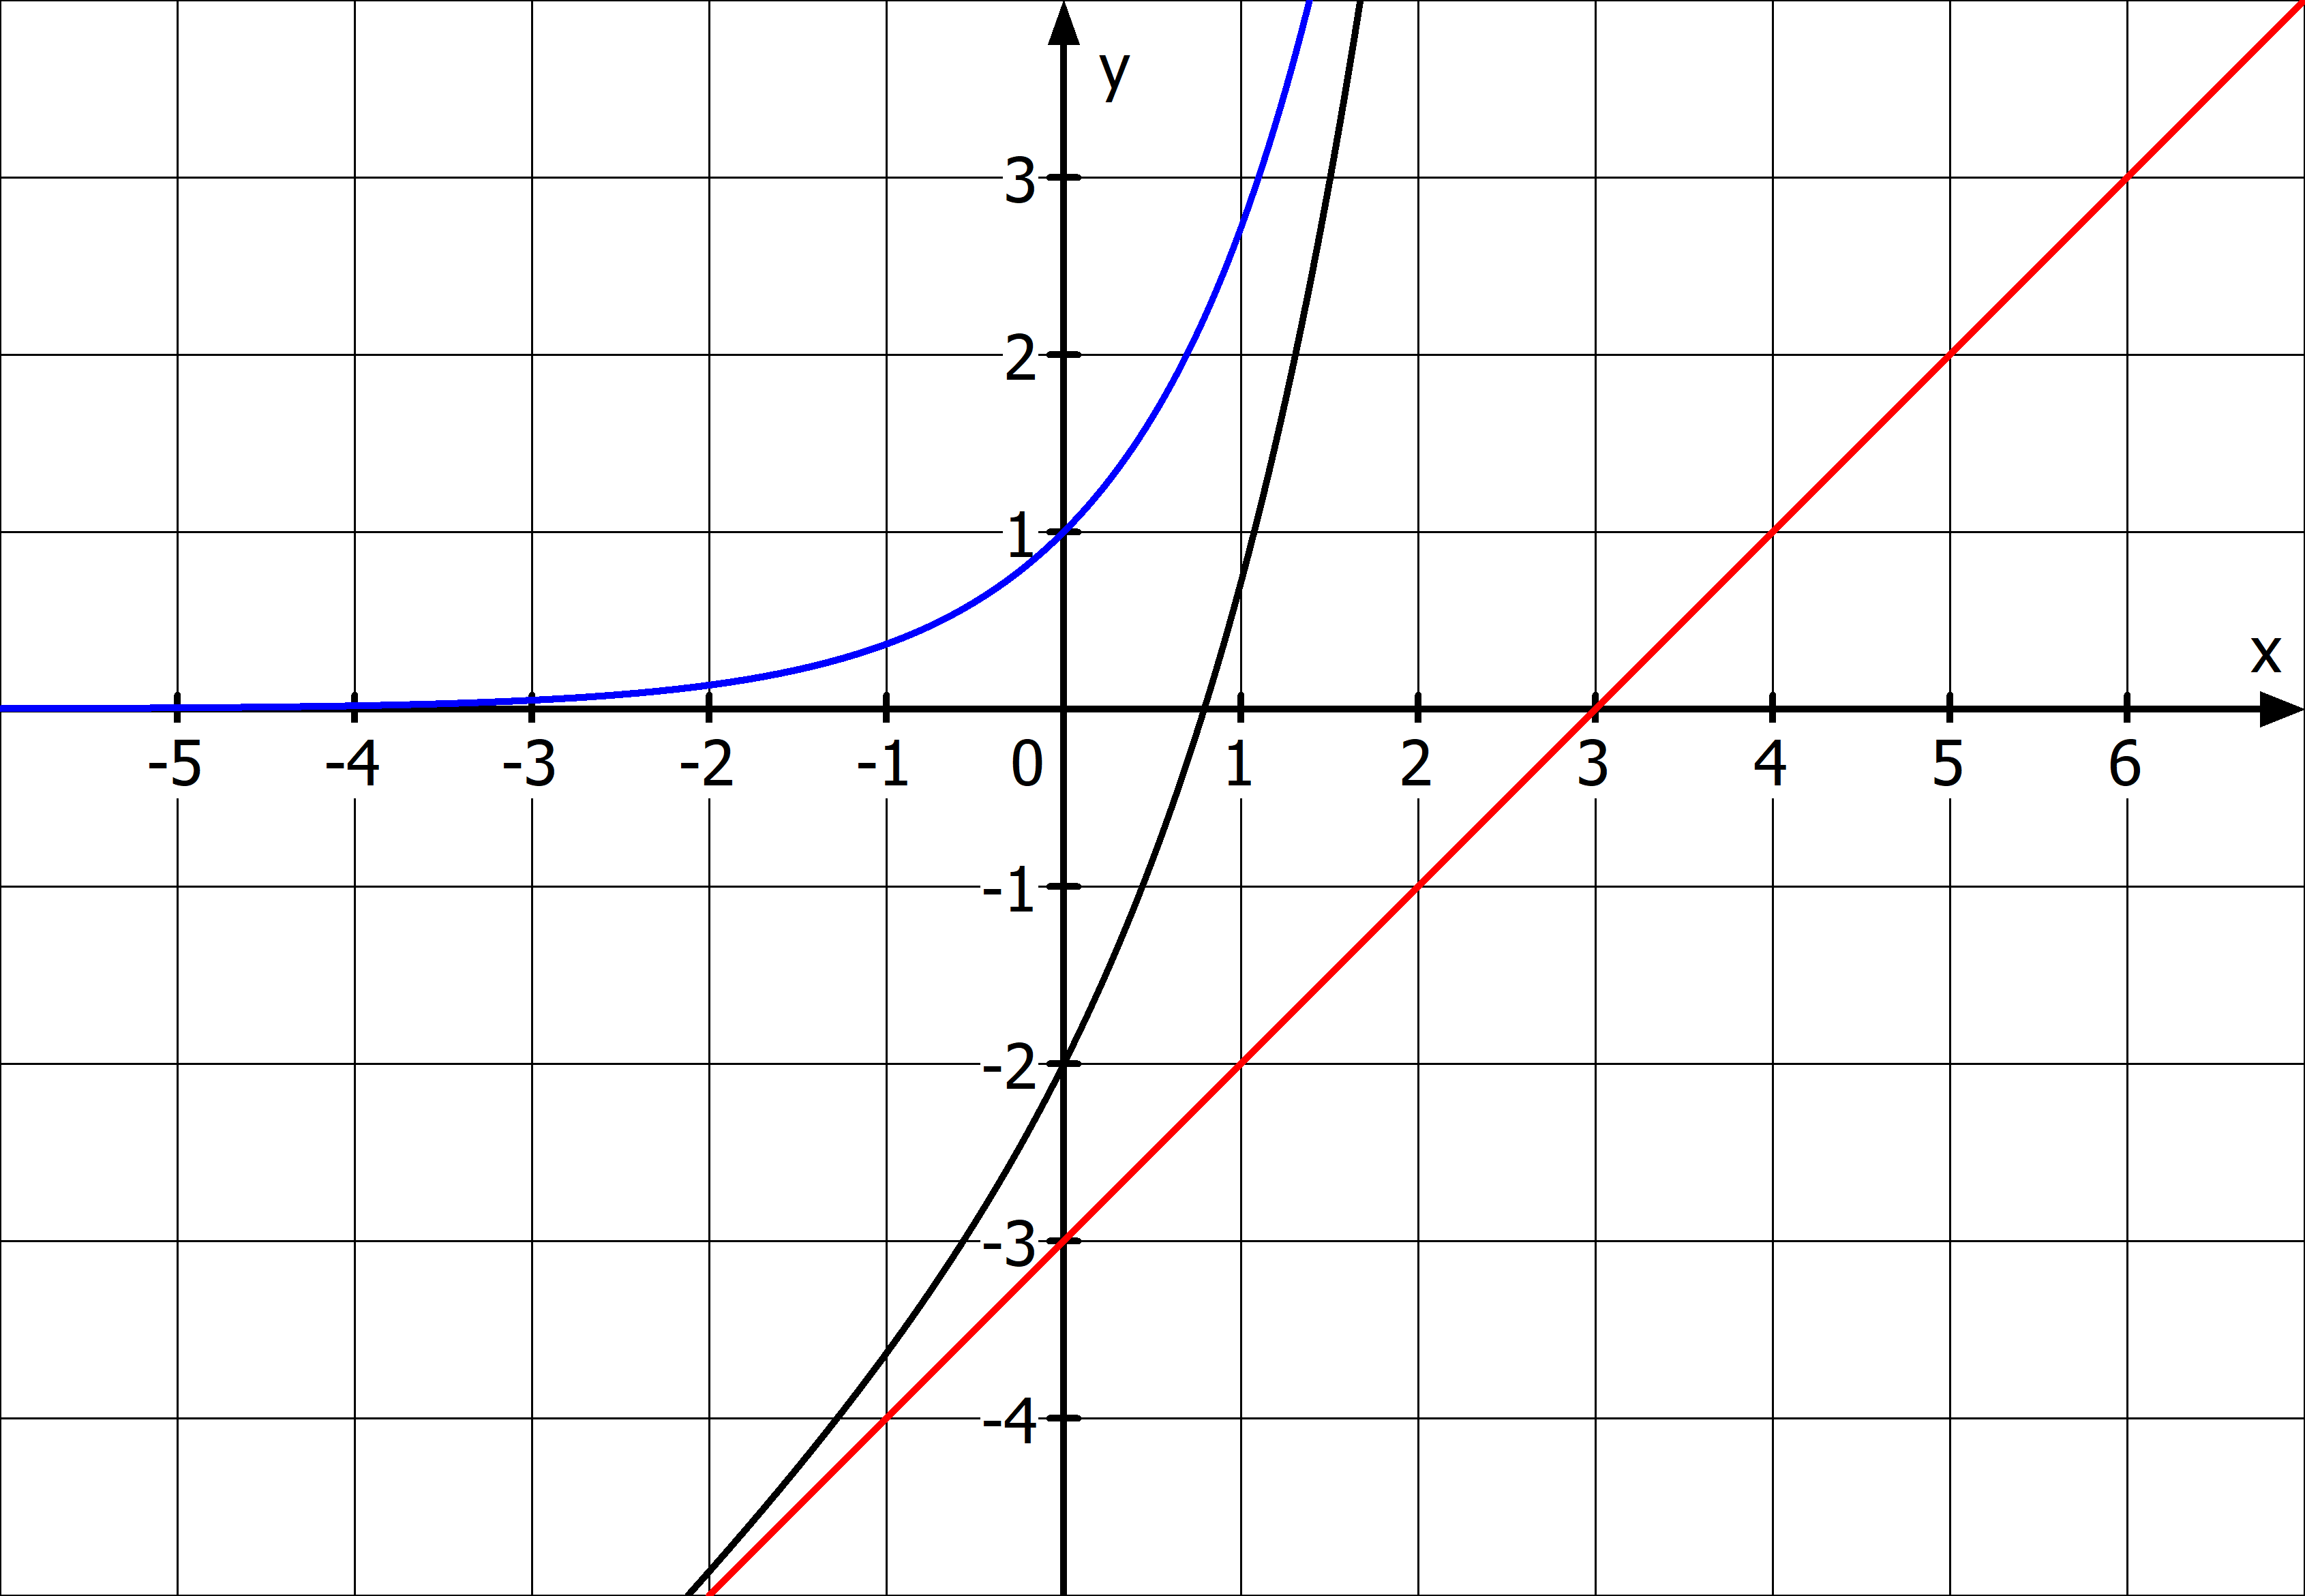
\includegraphics[width=\textwidth]{\eFkt/pics/Naeherungsweise.png}
    \end{minipage}}%
\end{minipage}

\medskip

Um die Nullstelle genauer zu bestimmen, gibt es verschiedene Verfahren wie z.B. das Newton-Verfahren. Wir werden einfach die Wertetabelle des Taschenrechners verwenden. In den Aufgaben ist normalerweise die Lage der Nullstelle bereits grob vorgegeben, z.B. \(f(x)=e^x+x-3\) hat zwischen \(x=0\) und \(x=1\) eine Nullstelle. Bestimme diese auf 2 Nachkommastellen genau. Wir erstellen eine Wertetabelle im Taschenrechner und geben als Startwert \(x=0\) an (als Endwert, soweit notwendig, \(x=1\)) und als Schrittweite (oft als step oder Inkrement bezeichnet) \(\Delta x=0,05\) an. Nun prüfen wir, an welcher Stelle der Vorzeichenwechsel stattfindet. Aus \(f(0,75)\approx -0,13\) und \(f(0,8)\approx 0,03\) folgt, dass die Nullstelle zwischen \(x=0,75\) und \(x=0,8\) liegen muss. Nun verfeinern wir die Wertetabelle mit Start \(x=0,75\) (Ende \(x=0,8\)) und Schrittweite \(\Delta x=0,005\) und erhalten aus \(f(0,79)\approx -0,007\) und \(f(0,795)\approx 0,009\) die ungefähre Lage der Nullstelle als \(x_1\approx 0,79\), da alle Werte zwischen 0,79 und 0,795 beim Runden auf die 2. Nachkommastelle auf 0,79 gerundet werden.

Mit dem gleichen Prinzip lassen sich auch die Nullstellen von Funktionen wie z.B.

\(f(x)=x^4-2x^3-4x+2\) bestimmen (\(x_1\approx 0,46\quad x_2\approx 2,51\)).

\begin{Exercise}[title={Prüfe an Hand deiner Skizze, ob die Funktionen aus Aufg. \ref{schAsyA1} NST haben und bestimme diese auf 2 Nachkommastellen genau.}, label=NSTnaeherungA1]
\end{Exercise}

%%%%%%%%%%%%%%%%%%%%%%%%%%%%%%%%%%%%%%%%%
\begin{Answer}[ref=NSTnaeherungA1]

	\begin{minipage}{\textwidth}
		\begin{minipage}{0.49\textwidth}
			\begin{enumerate}[label=\alph*)]
				\item \(f_1(x)=e^{-x}+2x-3\)

				\(x_1\approx 1,37\quad x_2\approx -1,92\)
				\item \(f_2(x)=-e^{-2x}+0,5x\)

				\(x_1\approx 0,60\)
				\item \(f_3(x)=-e^{x}-\frac{2}{3}x+1\)

				\(x_1=0\) (Exakte Lösung, da diese NST zufälligerweise exakt bestimmbar ist)
				\item \(f_4(x)=-2e^{-x}-2x+1\)

				keine Nullstellen
			\end{enumerate}
		\end{minipage}
		\begin{minipage}{0.49\textwidth}
			\begin{enumerate}[label=\alph*)]
				\setcounter{enumi}{4}
				\item \(f_5(x)=3e^{1,4x}+\frac{3}{4}x-1\)

				\(x_1\approx -0,54\)
				\item \(f_6(x)=e^{2x}+0,4x-3\)

				\(x_1\approx 0,51\)
				\item \(f_7(x)=-3e^{-0,5x}-x\)

				keine Nullstellen
				\item \(f_8(x)=-2e^{4x}+\frac{4}{3}x+5\)

				\(x_1\approx -3,75\quad x_2\approx 0,24\)
			\end{enumerate}
		\end{minipage}
	\end{minipage}
\end{Answer}